\documentclass{article}

\usepackage{subcaption}
\usepackage{graphicx}
\usepackage[utf8]{inputenc}
\usepackage[T1]{fontenc}
\usepackage[frenchb]{babel}

\begin{document}

\title{Rendu Projet Technologique}
\author{Zoe Debaty, Cedric Jolly, John Hermant, Mamodhoussen Bourhanoudine}
\maketitle

\newpage

\tableofcontents

\newpage

\section{Spécificités techniques}
\subsection{L'image}

\begin{center}
    \underline{\textbf{Multicolor}}
    \medbreak
    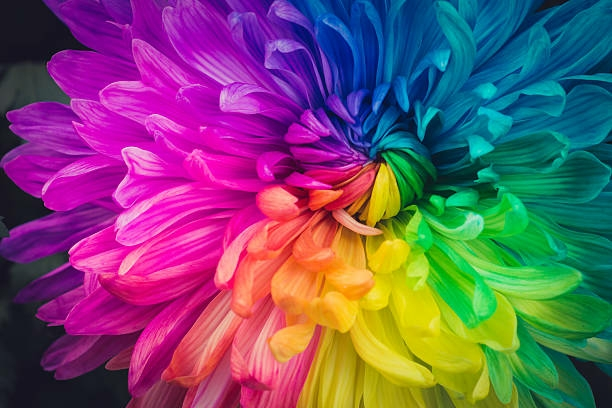
\includegraphics[width=300px]{./Images/Multicolor/base.jpg}
    \bigbreak
    \begin{itemize}
        \item Nom : "Multicolor"
        \item Dimensions : 612p * 408p
        \item Taille : 61,3 Ko
    \end{itemize}
\end{center}

L'image a été choisie car elle possède des changements de luminosité et énormément de couleurs afin de tester au mieux les fonctions.
Une fois dans l'application, il sera possible de zoomer dans l'image.

\subsection{Les téléphones}

Pour tester nos fonctionnalités, nous avons utilisés nos téléphones personnels :
\begin{itemize}
    \item Galaxy Note 8 (Android 9)
    \item Sony Xperia XZ1 (Android 9)
    \item Xiaomi mia3 (Android 9)
\end{itemize}
Ainsi que l'émulateur (Pixel 2 API 29 Android 10) et les Nokia de l'Université afin de vérifier que tout fonctionne peut importe le matériel utilisé. 
Les fonctions appliquées sur l'images "Multicolor" (images et temps) sont faites sur le Xperia. 
\newpage

\section{Fonctions}

Pour cette partie, nous decrierons les fonctions implémentées dans l'application et leur temps sera mentionné dans chaques cas. Si le langage n'est pas précisé, cela signifie que c'est une fonctions ecrite en JAVA.

\subsection{Griser l'image}
\medbreak

Cette fonctions passe une image RGB en teintes de gris
\medbreak

\subsubsection{JAVA}
\medbreak

\begin{center}
    \medbreak
    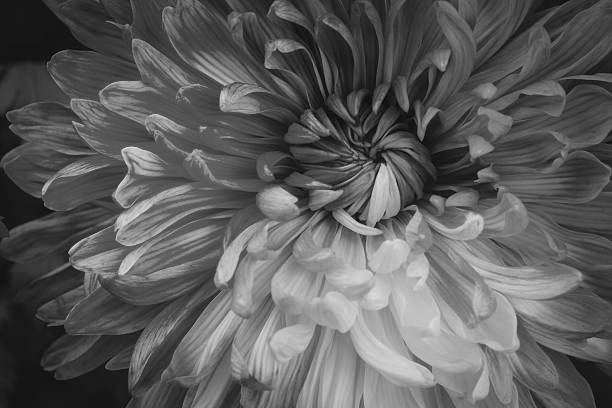
\includegraphics[width=300px]{./Images/Multicolor/Gray.jpg}
    \bigbreak
    Temps : 10,93 ms
\end{center}

\bigbreak
\subsubsection{Renderscript}
\medbreak

\begin{center}
    \medbreak
    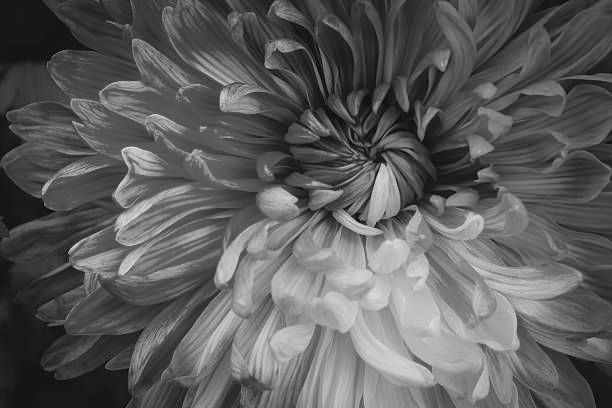
\includegraphics[width=300px]{./Images/Multicolor/Gray_RS.jpg}
    \bigbreak
    Temps au premier lancement : 147,96 ms
    \medbreak
    Temps au deuxième lancement : 11,73 ms
\end{center}

\bigbreak

\subsection{Coloriser l'image}
\medbreak

Cette fonctions colore une image RGB avec une couleur aléatoire. Il est aussi possible de modifier la teinte grâce à une seekBar
\medbreak

\begin{figure}[h!]
    \centering
    \begin{subfigure}[b]{0.4\linewidth}
        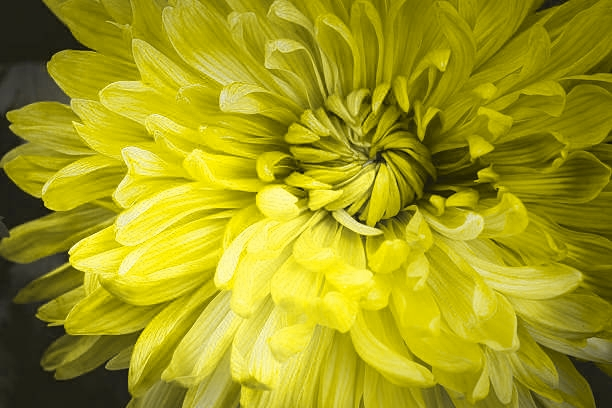
\includegraphics[width=\linewidth]{./Images/Multicolor/Random_1.jpg}
    \end{subfigure}
    \begin{subfigure}[b]{0.4\linewidth}
        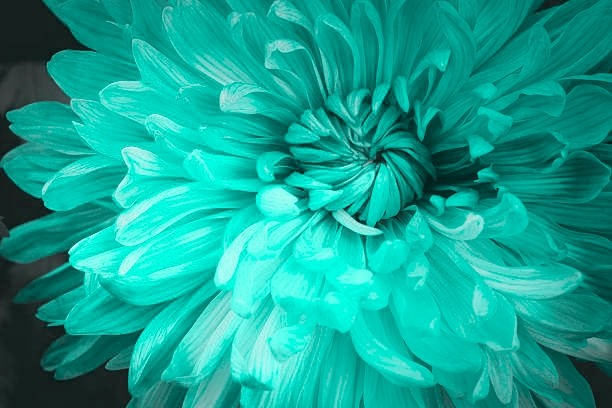
\includegraphics[width=\linewidth]{./Images/Multicolor/Random_2.jpg}
    \end{subfigure}
    \bigbreak
    Temps : 482,54 ms
\end{figure}

\subsection{Garder une ou plusieurs couleurs}
\medbreak

Cette fonction permet, au moyen de deux seekBar (qui vont contrôler respectivement la quantité de couleurs gardées et quelles couleurs) de garder les couleurs voulues sur l'image.
\medbreak

\subsubsection{JAVA}
\medbreak

\begin{center}
    \medbreak
    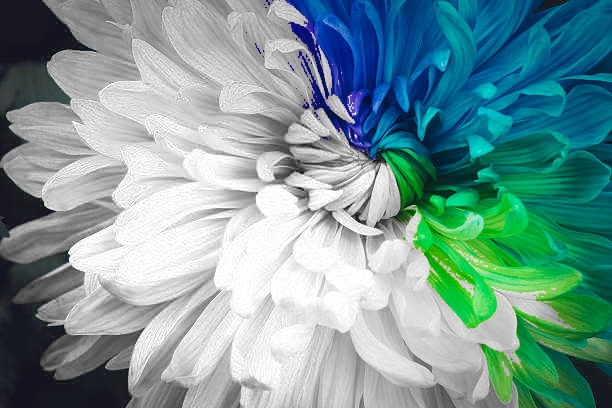
\includegraphics[width=300px]{./Images/Multicolor/Keep_Color.jpg}
    \bigbreak
    Temps  : 498,54 ms
\end{center}

\bigbreak

\subsubsection{Renderscript}
\medbreak

\begin{center}
    \medbreak
    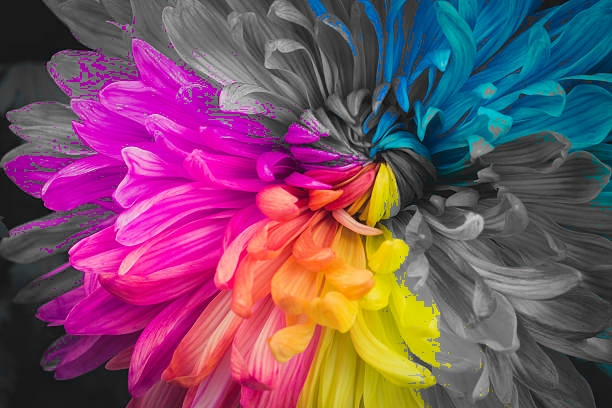
\includegraphics[width=300px]{./Images/Multicolor/Keep_Color_RS.jpg}
    \bigbreak
    Temps au premier lancement : 96,28 ms
    \medbreak
    Temps au deuxième lancement : 14,81 ms
\end{center}

\bigbreak
\subsection{Extension de dynamique}
\medbreak

Cette fonction applique une extension de dynamique sur une image RGB.
\medbreak

\begin{figure}[h!]
    \centering
    \begin{subfigure}[b]{0.4\linewidth}
        Sur une image en couleur
        \medbreak
        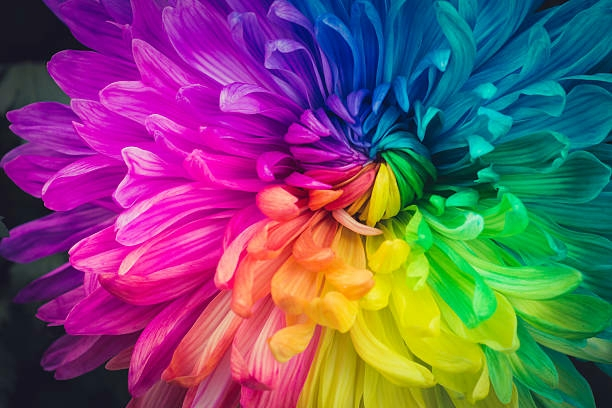
\includegraphics[width=\linewidth]{./Images/Multicolor/Color_Linear_Extension.jpg}
    \end{subfigure}
    \begin{subfigure}[b]{0.4\linewidth}
        Sur une image en teintes de gris
        \medbreak
        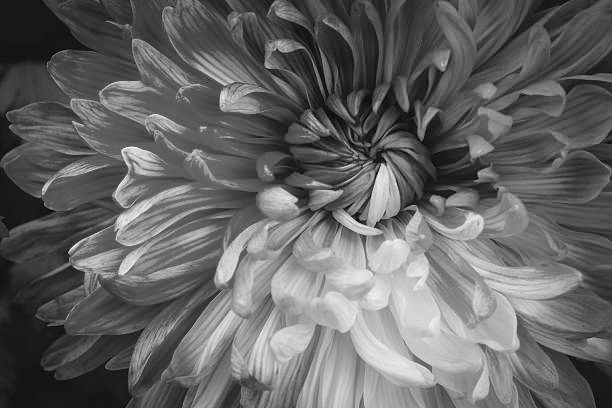
\includegraphics[width=\linewidth]{./Images/Multicolor/Gray_Linear_Extension.jpg}
    \end{subfigure}
    \bigbreak
    Temps  : 26,06 ms
\end{figure}

\bigbreak
\subsection{Egalisation d'histogramme}
\medbreak

Cette fonction applique une égalisation d'histogramme sur une image RGB.
\medbreak

\begin{figure}[h!]
    \centering
    \begin{subfigure}[b]{0.4\linewidth}
        Sur une image en couleur
        \medbreak
        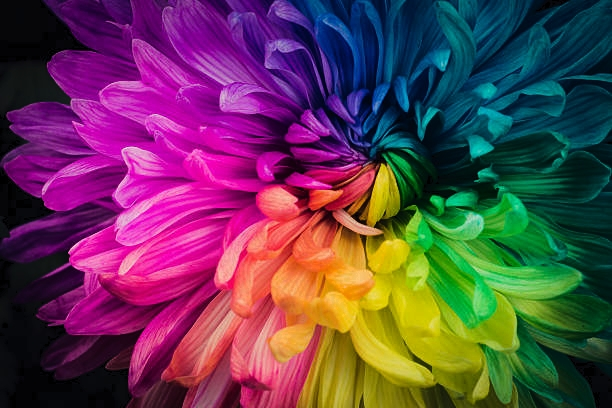
\includegraphics[width=\linewidth]{./Images/Multicolor/Color_Egalisation.jpg}
    \end{subfigure}
    \begin{subfigure}[b]{0.4\linewidth}
        Sur une image en teintes de gris
        \medbreak
        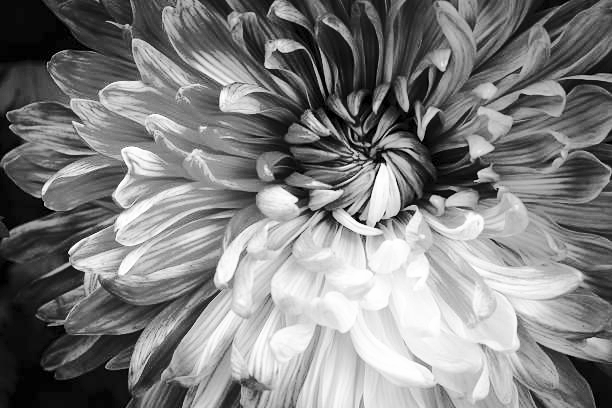
\includegraphics[width=\linewidth]{./Images/Multicolor/Gray_Egalisation.jpg}
    \end{subfigure}
    \bigbreak
    Temps  : 913,24 ms
\end{figure}

\bigbreak
\subsection{Moyenneur}
Cette fonction permet d'appliquer le filtre moyenneur sur l'image courante. Ce filtre est pour l'instant disponible en trois tailles :
\medbreak

-> 3x3
\begin{center}
    \medbreak
    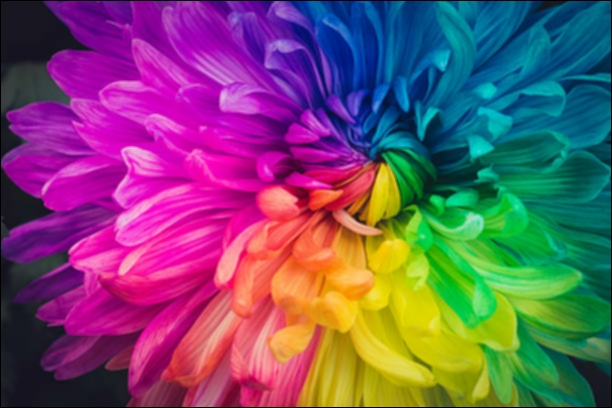
\includegraphics[width=300px]{./Images/Multicolor/Average_3.jpg}
    \bigbreak
    Temps  : 161,58 ms
\end{center}
\medbreak

-> 7x7
\begin{center}
    \medbreak
    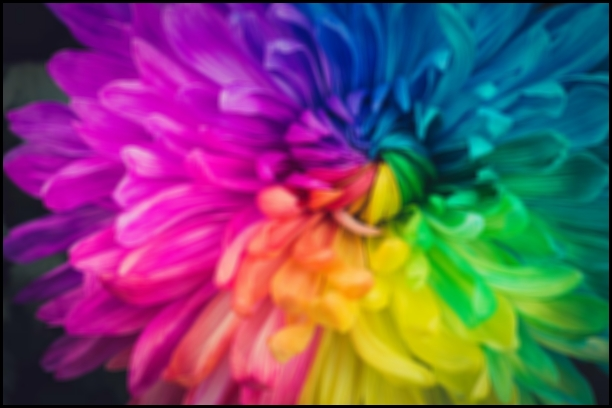
\includegraphics[width=300px]{./Images/Multicolor/Average_7.jpg}
    \bigbreak
    Temps  : 426,71 ms
\end{center}
\medbreak

-> 15x15
\begin{center}
    \medbreak
    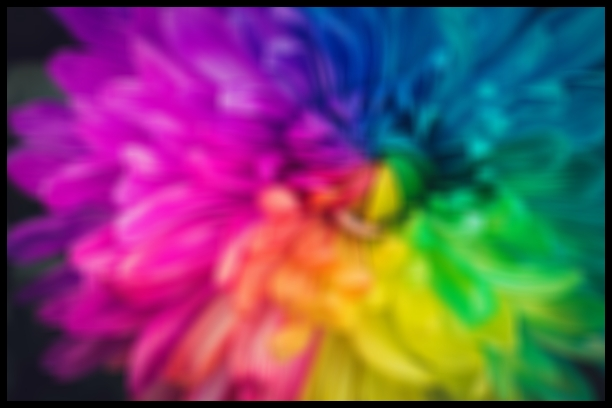
\includegraphics[width=300px]{./Images/Multicolor/Average_15.jpg}
    \bigbreak
    Temps  : 1720 ms
\end{center}
\bigbreak

\subsection{Gaussien}
Cette fonction permet d'appliquer le filtre Gaussien de taille 5x5 sur l'image courante.
\medbreak

\begin{center}
    \medbreak
    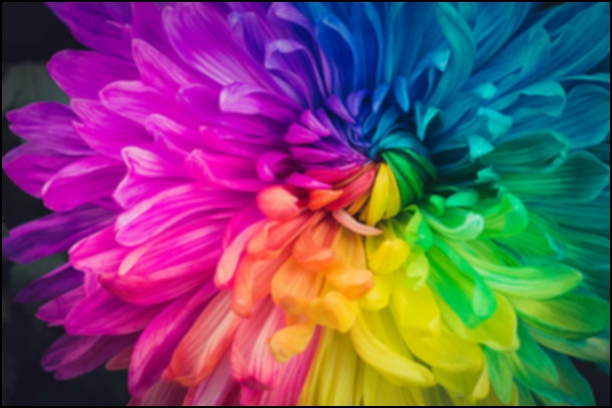
\includegraphics[width=300px]{./Images/Multicolor/Gaussian_15.jpg}
    \bigbreak
    Temps  : 233,58 ms
\end{center}
\bigbreak

\subsection{Prewitt}
Cette fonction permet d'appliquer le filtre utilisant l'opérateur de Prewitt sur l'image courante.
\medbreak

-> Horizontal
\begin{center}
    \medbreak
    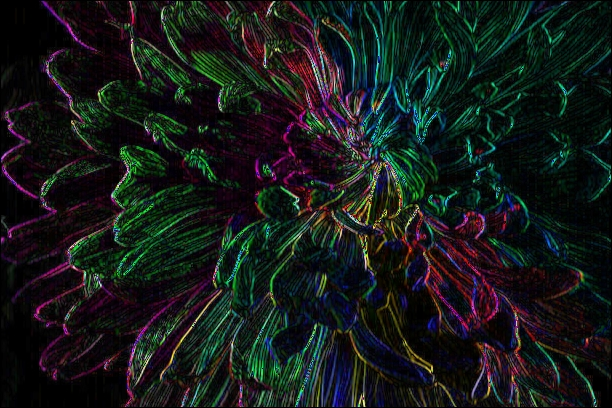
\includegraphics[width=300px]{./Images/Multicolor/Prewitt_Hor.jpg}
    \bigbreak
    Temps  : 154,19 ms
\end{center}
\medbreak

-> Vertical
\begin{center}
    \medbreak
    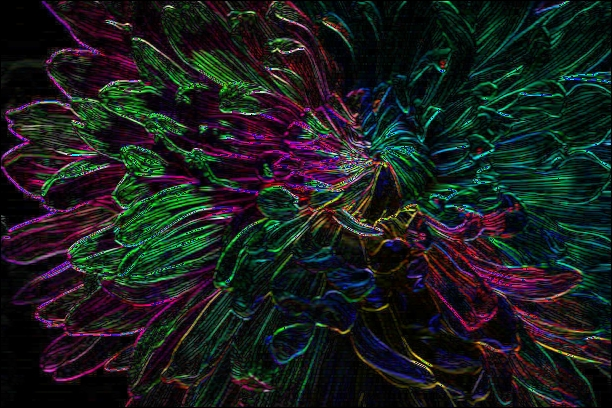
\includegraphics[width=300px]{./Images/Multicolor/Prewitt_Ver.jpg}
    \bigbreak
    Temps  : 116,58 ms
\end{center}
\medbreak

-> Tout
\begin{center}
    \medbreak
    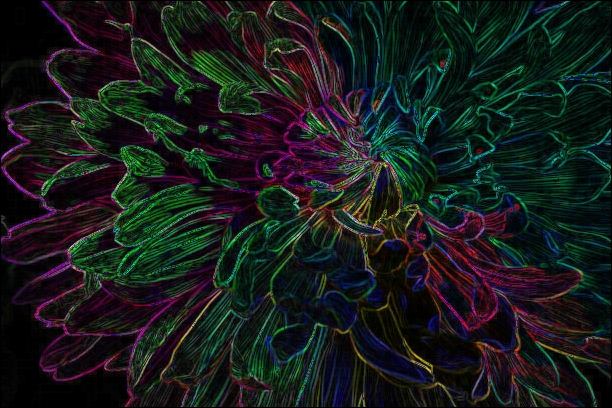
\includegraphics[width=300px]{./Images/Multicolor/Prewitt_All.jpg}
    \bigbreak
    Temps  : 231,04 ms
\end{center}
\bigbreak

\subsection{Sobel}
Cette fonction permet d'appliquer le filtre utilisant l'opérateur de Sobel sur l'image courante.
\medbreak

-> Horizontal
\begin{center}
    \medbreak
    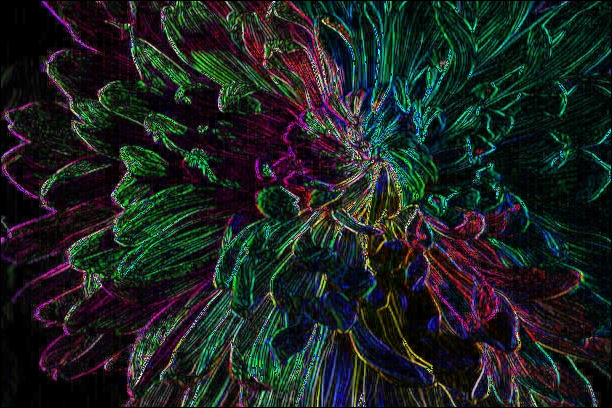
\includegraphics[width=300px]{./Images/Multicolor/Sobel_Hor.jpg}
    \bigbreak
    Temps  : 112,59 ms
\end{center}
\medbreak

-> Vertical
\begin{center}
    \medbreak
    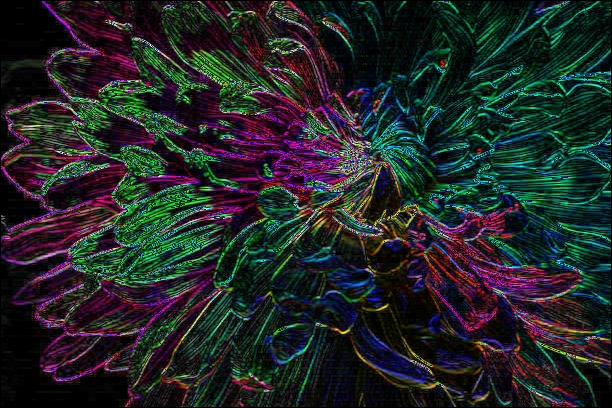
\includegraphics[width=300px]{./Images/Multicolor/Sobel_Ver.jpg}
    \bigbreak
    Temps  : 110,85 ms
\end{center}
\medbreak

-> Tout
\begin{center}
    \medbreak
    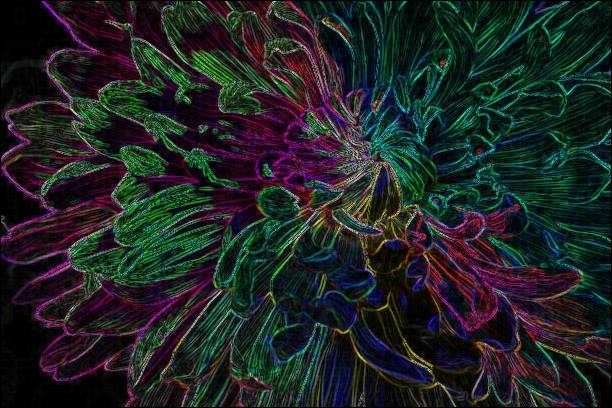
\includegraphics[width=300px]{./Images/Multicolor/Sobel_All.jpg}
    \bigbreak
    Temps  : 239,44 ms
\end{center}
\bigbreak

\subsection{Laplacien}
Cette fonction permet d'appliquer le filtre utilisant l'opérateur de Laplacien sur l'image courante.
\medbreak

-> 4 cx
\begin{center}
    \medbreak
    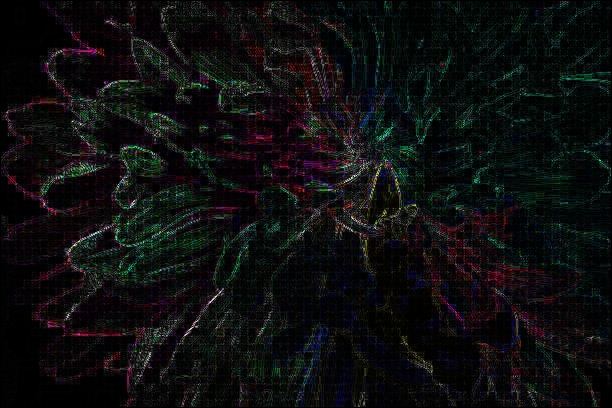
\includegraphics[width=300px]{./Images/Multicolor/Laplacian_4.jpg}
    \bigbreak
    Temps  : 121,9 ms
\end{center}
\medbreak

-> 8 cx
\begin{center}
    \medbreak
    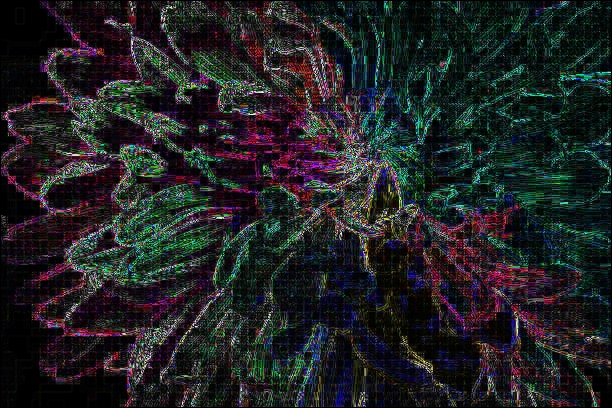
\includegraphics[width=300px]{./Images/Multicolor/Laplacian_8.jpg}
    \bigbreak
    Temps  : 113,61 ms
\end{center}
\medbreak

\subsection{Negatif}
Cette fonction passe une image RGB en négatif.
\medbreak

\begin{center}
    \medbreak
    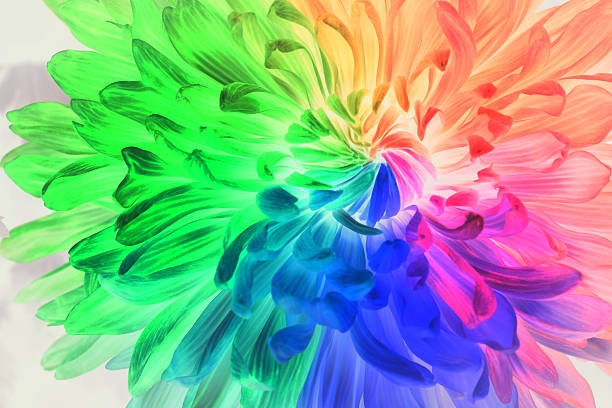
\includegraphics[width=300px]{./Images/Multicolor/Negative.jpg}
    \bigbreak
    Temps  : 12,72 ms
\end{center}
\bigbreak

\subsection{Saturation}
Cette fonction permet de modifier la saturation d'une image RGB au moyen d'une seekBar.
\medbreak

\begin{center}
    \medbreak
    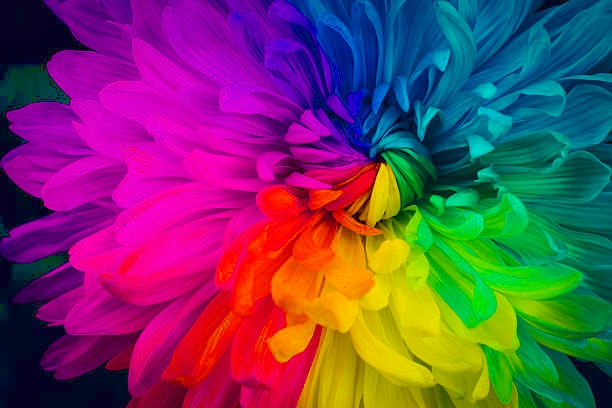
\includegraphics[width=300px]{./Images/Multicolor/Saturation_Max.jpg}
    \bigbreak
    Temps  : 539,3 ms
\end{center}
\bigbreak

\subsection{Luminosité}
Cette fonction permet de modifier la luminosité d'une image RGB au moyen d'une seekBar.
\medbreak

\begin{center}
    \medbreak
    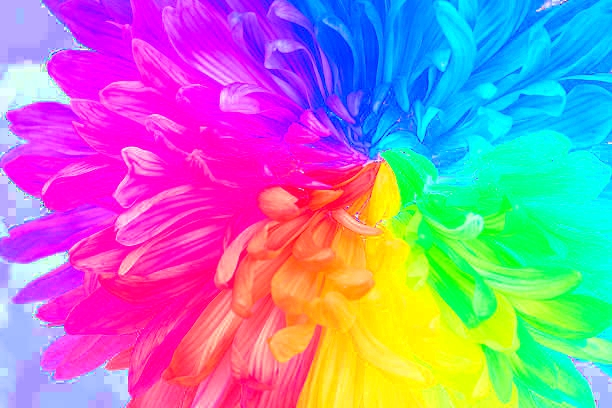
\includegraphics[width=300px]{./Images/Multicolor/Brightness_Max.jpg}
    \bigbreak
    Temps  : 484,58 ms
\end{center}
\bigbreak

\subsection{HSV <-> RGB}
Ces fonctions permettent de passer d'une image RGB en une image hsv et inversement. Afin de tester leurs performances, je les aient appelé à la suite et j'ai comparé le résultat aux fonctions de base de la librairie Colors.
\medbreak
Temps (librairie Colors) : 11 080 625
\medbreak
Temps (nos fonctions) : 927 161

\subsection{Fonctions pratiques}
\subsubsection{Sauvegarder}
Cette fonction permet de sauvegarder l'image courante. Son temps d'application est de 1ms.
\bigbreak

\subsubsection{Charger depuis la gallerie}
Cette fonciton permet de charger depuis la gallerie du téléphone. Son temps d'application est de 53,27 ms.
\bigbreak

\subsubsection{Charger depuis la caméra}
Cette fonciton permet de prendre une image depuis la caméra et de la charger. Nous n'avons pas pu connaître son temps d'applicatio car ce dernier depend du temps passé dans l'application caméra.

\section{Organisation du code}
\subsection{MainActivity}
\medbreak

Classe principale où l'application se lance. Déclaration des attributs et mise en place de l'interface utilisateur de l'application. C'est dans cette classe que tous les appels aux classes intermédiaires se font (Notamment les classes d'algorithme). Dans cette classe la gestion de la caméra et de la galerie est paramétrée.
\bigbreak

\subsection{Package Algorithms}
Ce package contient nos fonctions pour les algorithmes.
\subsubsection{Functions}
\medbreak

Cette classe contient majoritairement les algorithmes de traitement d'image classique ne demandant pas leurs propres attributs. Elle contient les algorithmes suivants: toGray, colorize, keepColor, change\_saturation, change\_brightness, negative.
\medbreak

\subsubsection{FunctionsRS}
\medbreak

Classe similaire à celle indiquée précédemment, à l'exception qu'elle supporte uniquement les fonctions écrites en RenderScript. Cependant elles contiennent pour le moment que les fonctions toGray et keepColor.
\medbreak

\subsubsection{Tools}
\medbreak

Classe "outils" qui contient des algorithmes utilisés presque systématiquement dans nos algorithmes de traitement d'image comme par exemple la conversion RGB vers HSV et vice versa, récupérer le min et le max de chaque canal de couleur RGB, le calcul d'histogramme et le calcul d'histogramme cumulatif.
\medbreak

\subsubsection{Contrast}
\medbreak

Cette classe permet d'effectuer l'algorithme de contraste avec la transformation linéaire en créant les LookUP Table des canaux RGB.
\medbreak

\subsubsection{Convolution}
\medbreak

Cette classe contient plusieurs filtres applicables avec le principe de convolution. Les filtres disponibles sont: Moyenneur, Gaussien, Prewitt, Sobel et Laplacien.
\medbreak

\section{Autre}
\subsection{Bugs connus}

\begin{itemize}
    \item Rotation automatique des images récupérées depuis la galerie ou pris avec la caméra
    \item Convolution -> Sobel et Prewitt ne donnent pas forcément le résultat recherché.
    \item keepColor en version Renderscript ne possède pas la meme plage de couleur que la version JAVA. Son passage en gris n'est pas le même non plus.
\end{itemize}

\subsection{Améliorations}

Notre priorité sera de corriger les bugs et de pouvoir avoir toutes les fonctions en Renderscript, après cela, nous pourront voir les améliorations suivantes :

\begin{itemize}
    \item Améliorer la structure du code -> ajout d'une classe Intent (Caméra, Gallerie)
    \item Améliorer le design de l'application
    \item Ajout d'options -> autocollant, rogner l'image, ajout de texte, dessiner, effectuer des rotations
    \item Permettre à l'utilisateur d'avoir un historique de ses actions permettant des retours en arrières
    \item Ajout de nouveaux filtres (Sépia par exemple)
    \item Ajout de seekBar pour certaines fonctions
    \item Avoir des filtres gaussien de plusieurs tailles
\end{itemize}

\subsection{Autorisations}

A la première ouverture de l'application, des autorisations sont demandées pour pouvoir écrire ou lire le stockage de l'appareil et pour pouvoir utiliser l'application.
Si elles sont refusées, ces autorisations sont redemandées au moment où l'on essaie de sauvegarder une image, prendre une photo ou en récupérer une depuis la galerie.

Caméra: L'image prise est enregistrée dans l'appareil et est ensuite chargée.

Galerie: L'image est récupérée directement depuis le stockage interne

Save: L'image est enregistrée dans le dossier piceditor dans la mémoire interne.

\end{document}